\documentclass[12pt]{article}
\usepackage{amsmath, amsthm, amssymb}
\usepackage[top=1.25in, bottom=1.25in, left=1.0in, right=1.0in]{geometry}
\usepackage{hyperref}
\usepackage{color}
\usepackage{verbatim}
\usepackage{tikz,tkz-graph}

\makeatletter
\newtheorem*{rep@theorem}{\rep@title}
\newcommand{\newreptheorem}[2]{
\newenvironment{rep#1}[1]{
 \def\rep@title{#2 \ref{##1}}
 \begin{rep@theorem}}
 {\end{rep@theorem}}}
\makeatother

\theoremstyle{plain}
\newtheorem{thm}{Theorem}
\newreptheorem{thm}{Theorem}
\newtheorem{prop}[thm]{Proposition}
\newreptheorem{prop}{Proposition}
\newtheorem{lem}[thm]{Lemma}
\newreptheorem{lem}{Lemma}
\newtheorem{lemma}[thm]{Lemma}
\newtheorem*{lemmaA}{Tashkinov's Lemma}
\newtheorem*{PEL}{Parallel Edge Lemma}
\newtheorem*{GS}{Goldberg--Seymour Conjecture}
\newtheorem*{main}{Theorem 16}
\newtheorem*{main2}{Theorem 13}
\newreptheorem{lemma}{Lemma}
\newtheorem{conj}[thm]{Conjecture}
\newreptheorem{conj}{Conjecture}
\newtheorem{cor}[thm]{Corollary}
\newreptheorem{cor}{Corollary}
\newtheorem{prob}[thm]{Problem}
\theoremstyle{definition}
\newtheorem{defn}{Definition}
\newtheorem{clm}{Claim}
\newtheorem{obs}[thm]{Observation}
\theoremstyle{remark}
\newtheorem*{remark}{Remark}
\newtheorem{example}{Example}
\newtheorem*{question}{Question}

\newcommand{\fancy}[1]{\mathcal{#1}}
%\newcommand{\C}[1]{\fancy{C}_{#1}}
\newcommand{\C}{\fancy{C}}
\newcommand{\F}{\fancy{F}}
\newcommand{\W}{\fancy{W}}
\newcommand{\IN}{\mathbb{N}}
\newcommand{\IR}{\mathbb{R}}
\newcommand{\G}{\fancy{G}}
\newcommand{\B}{\fancy{B}}
\newcommand{\LB}{\mathcal{L}_B}
\newcommand{\col}{{\textrm{col}}}
\newcommand{\ch}{{\textrm{ch}}}
\newcommand{\chil}{{\chi_{\ell}}}
\newcommand{\chiol}{{\chi_{OL}}}
\newcommand{\T}{\fancy{T}}

\newcommand{\inj}{\hookrightarrow}
\newcommand{\surj}{\twoheadrightarrow}

\newcommand{\set}[1]{\left\{ #1 \right\}}
\newcommand{\setb}[3]{\left\{ #1 \in #2 : #3 \right\}}
\newcommand{\setbs}[2]{\left\{ #1 : #2 \right\}}
\newcommand{\card}[1]{\left|#1\right|}
\newcommand{\size}[1]{\left\Vert#1\right\Vert}
\newcommand{\ceil}[1]{\left\lceil#1\right\rceil}
\newcommand{\floor}[1]{\left\lfloor#1\right\rfloor}
\newcommand{\func}[3]{#1\colon #2 \rightarrow #3}
\newcommand{\funcinj}[3]{#1\colon #2 \inj #3}
\newcommand{\funcsurj}[3]{#1\colon #2 \surj #3}
\newcommand{\irange}[1]{\left[#1\right]}
\newcommand{\join}[2]{#1 \mbox{\hspace{2 pt}$\ast$\hspace{2 pt}} #2}
\newcommand{\djunion}[2]{#1 \mbox{\hspace{2 pt}$+$\hspace{2 pt}} #2}
\newcommand{\parens}[1]{\left( #1 \right)}
\newcommand{\brackets}[1]{\left[ #1 \right]}
\newcommand{\DefinedAs}{\mathrel{\mathop:}=}

\newcommand{\mic}{\operatorname{mic}}
\newcommand{\AT}{\operatorname{AT}}
\renewcommand{\col}{\operatorname{col}}
\renewcommand{\ch}{\operatorname{ch}}
\newcommand{\type}{\operatorname{type}}
\newcommand{\nonsep}{\bar{S}}
\newcommand{\dclaw}[1]{d_{\text{claw}}\left( #1 \right)}

\def\adj{\leftrightarrow}
\def\nonadj{\not\!\leftrightarrow}

\newcommand{\vph}{\varphi}
\newcommand{\vphn}{\overline{\varphi}}

\newcommand{\claim}[2]{{\noindent\bf Claim #1.}~{\it #2}~~}
\newenvironment{claimproof}[1]{\par\noindent\underline{Proof:}\space#1}{\leavevmode\unskip\penalty9999
\hbox{}\nobreak\hfill\quad\hbox{$\qed$}}
%
%  If the proof ends with a displayed equation, use \aftermath just
%  before \end{proof} to put the halmos in the ``right'' place.  This
%  may not work near page boundaries. 
%
\def\aftermath{\par\vspace{-\belowdisplayskip}\vspace{-\parskip}\vspace{-\baselineskip}}

\title{Short fans and the 5/6 bound for line graphs}
\author{Daniel W. Cranston\and Landon Rabern}

\begin{document}
\maketitle
\begin{abstract}
In 2011, the second author conjectured that every line graph $G$ satisfies
$\chi(G)\le \max\set{\omega(G),\frac{5\Delta(G)+8}{6}}$. This conjecture is best
possible, as shown by replacing each edge in a 5-cycle by $k$ parallel edges,
and taking the line graph. In this paper we prove the conjecture.
We also develop more general techniques and results that will likely be of
independent interest, due to their use in attacking the Goldberg--Seymour
conjecture.  
\end{abstract}

\section{Overview}

By \emph{graph} we mean multigraph without loops.  Our notation follows Diestel
\cite{diestel2010}.
In \cite{rabern2011strengthening}, the second author showed that $\chi(G)\le
\max\set{\omega(G), \frac{7\Delta(G)+10}{8}}$ for every line graph $G$.
In the same paper, he conjectured
that $\chi(G)\le \max\set{\omega(G),\frac{5\Delta(G)+8}{6}}$. This conjecture is best
possible, as shown by replacing each edge in a 5-cycle by $k$ parallel edges,
and taking the line graph. In this paper we prove the latter inequality.  Along
the way, we develop more general techniques and results that will likely be of
independent interest.  The main result of this paper is the following theorem.
\begin{main}[$\frac56$-Theorem]
If $Q$ is a line graph, then 
\[\chi(Q)\le \max\set{\omega(Q),\frac{5\Delta(Q)+8}{6}}.\]
\end{main}

For every graph $G$, we have $\chi'(G)\ge
\ceil{\frac{\size{G}}{\floor{\frac{\card{G}}{2}}}}$, since each color class has size at most
$\floor{\frac{\card{G}}{2}}$.  Likewise, the same bound holds for any subgraph $H$.  
Thus $\chi'(G)\ge \max_{H\subseteq G}\ceil{\frac{\size{H}}{\floor{\frac{\card{H}}{2}}}}$
(where the max is over all subgraphs $H$ with at least two vertices).
For convenience, we let $\W(G)\DefinedAs\max_{H\subseteq
G}\ceil{\frac{\size{H}}{\floor{\frac{\card{H}}{2}}}}$.
Goldberg~\cite{goldberg1973,GoldbergJGT} and
Seymour~\cite{seymour1979a,seymour1979b} each conjectured that this lower bound
holds with equality, whenever $\chi'(G)>\Delta(G)+1$.
\begin{GS}
Every graph $G$ satisfies
\[
\chi'(G)\le\max\{\W(G), \Delta(G)+1\}.
\]
\end{GS}
The Goldberg--Seymour conjecture is the major open problem in the area of
edge-coloring graphs.
Most of our work goes toward proving the following
intermediate result, in Section~\ref{sec:thin}.  
\begin{main2}[Weak $\frac56$-Theorem]
If $Q$ the line graph of a graph $G$, then 
\[\chi(Q)\le \max\set{\W(G),\Delta(G)+1,\frac{5\Delta(Q)+8}{6}}.\]
\end{main2}
Finally, in Section~\ref{sec:final} we show that the Weak $\frac56$-Theorem
does indeed imply the $\frac56$-Theorem.


\section{Tashkinov Trees}
A graph $G$ is \emph{elementary} if $\chi'(G)=\W(G)$. 
%as defined above.  
%We also use the following notation.  
Let $[k]$ denote $\{1,\ldots,k\}$.
For a path or cycle $Q$, let \emph{$\ell(Q)$} denote the length of $Q$.
A graph $G$ is \emph{critical} if $\chi'(G-e) < \chi'(G)$ for all $e \in E(G)$. 
For a graph $G$ and a partial $k$-edge-coloring $\varphi$, for each vertex $v\in
V(G)$, let $\varphi(v)$ denote the set of colors used in $\varphi$ on edges
incident to $v$.  Let $\vphn(v)=[k]\setminus\varphi(v)$.  A color $c$ is
\emph{seen} by a vertex $v$ if $c\in \varphi(v)$ and $c$ is \emph{missed} by $v$
if $c\in\vphn(v)$.
Given a partial $k$-edge-coloring $\varphi$, a set $W\subseteq V(G)$ is
\emph{elementary} with respect to $\varphi$ (henceforth,
\emph{w.r.t.~$\varphi$}) if each color in $[k]$ is
missed by at most one vertex of $W$.  More formally, $\vphn(u)\cap
\vphn(v)=\emptyset$ for all distinct $u,v\in W$.
A \emph{defective color} for a set $X\subseteq V(G)$ (w.r.t.~$\varphi$) is a color
used on more than one edge from $X$ to $V(G) \setminus X$.  
A set $X$ is \emph{strongly closed} w.r.t.~$\varphi$ if $X$ has no 
defective color.
Elementary and strongly closed sets are of particular interest because of the
following theorem, proved implicitly by Andersen~\cite{andersen1977edge} and
Goldberg~\cite{GoldbergJGT}; see also~\cite[Theorem 1.4]{SSTF}.
%As we will see shortly, there is a strong relationship between elementary sets
%and elementary graphs.
% 

\begin{thm}
\label{elementary}
Let $G$ be a graph with $\chi'(G)=k+1$ for some integer $k\ge \Delta(G)$.  If
$G$ is critical, then $G$ is elementary if and only if there exists $uv\in E(G)$,
a $k$-edge-coloring $\vph$ of $G-uv$, and a set $X$ with $u,v\in X$ such
that $X$ is both elementary and strongly closed w.r.t.~$\varphi$.
\end{thm}

A \emph{Tashkinov tree} w.r.t.~$\varphi$ is a sequence $v_0, e_1, v_1,
e_2,\ldots, v_{t-1},e_t,v_t$ such that all $v_i$ are distinct, $e_i=v_jv_i$ and
$\vph(e_i)\in \vphn(v_\ell)$ for some $j$ and $\ell$ with $0\le j< i$ and $0\le
\ell < i$.  
A \emph{Vizing fan} (or simply \emph{fan}) is a Tashkinov tree that induces a
star.  Tashkinov trees are of interest because of the following lemma. 

\begin{lemmaA}%[Tashkinov]
Let $G$ be a graph with $\chi'(G)=k+1$, for some integer $k\ge \Delta(G)+1$ and
choose $e\in E(G)$ such that $\chi'(G-e)<\chi'(G)$.  Let $\varphi$ be a
$k$-edge-coloring of $G-e$.  If $T$ is a Tashkinov tree w.r.t.~$\varphi$ and
$e$, then $V(T)$ is elementary w.r.t.~$\varphi$.
\end{lemmaA}

In view of Theorem~1 and Tashkinov's Lemma, to prove that a graph $G$ is elementary,
it suffices to find an edge $e$, a $k$-edge-coloring $\vph$ of $G-e$, and a
Tashkinov tree $T$ containing $e$ such that $V(T)$ is strongly closed.
This motivates our next two lemmas.  But first, we need a few more definitions.

Let $t(G)$ be the maximum number of vertices in a Tashkinov tree over all $e \in E(G)$
and all $k$-edge-colorings $\vph$ of $G - e$.  Let $\T(G)$ be the set of all triples $(T,e,\vph)$ such that $e \in E(G)$, $\vph$ is a $k$-edge-coloring of $G-e$ and
$T$ is a Tashkinov tree with respect to $e$ and $\vph$ with $|T| = t(G)$.  Notice that, by definition, we have $\T(G) \ne \emptyset$.
%
For a $k$-edge-coloring $\vph$ of $G-e$, a maximal Tashkinov tree
starting with $e$ may not be unique.  However, if $T_1$ and $T_2$ are both such
trees, then it is easy to show that $V(T_1)\subseteq V(T_2)$; by symmetry, also
$V(T_2)\subseteq V(T_1)$, so $V(T_1)=V(T_2)$.
%
Let $G$ be a critical graph with $\chi'(G) = k+1$ for some integer $k \ge \Delta(G) + 1$. 
Let $\varphi$ be a $k$-edge-coloring of $G - e_0$ for some $e_0 \in E(G)$.  
%For each vertex $v\in V(G)$, let $\varphi(v)$ be the set of colors used in
%$\vph$ on edges incident to $v$ and let $\vphn(v)=[k]\setminus \vph(v)$. 
For $v \in V(G)$ and colors $\alpha, \beta$, let $P_v(\alpha, \beta)$ be the
maximal connected subgraph of $G$ that contains $v$ and is induced by edges with color
$\alpha$ or $\beta$.  So $P_v(\alpha, \beta)$ is a path or a cycle.
For a $k$-edge-coloring $\vph$ of $G-v_0v_1$, we often let
$P=P_{v_1}(\alpha,\beta)$ for some $\alpha\in\vphn(v_0)$ and
$\beta\in\vphn(v_1)$.  
Clearly $P$ must end at $v_0$ (or we can swap colors $\alpha$ and $\beta$ on
$P$ and color $v_0v_1$ with $\alpha$), so let $v_1,\ldots,v_r,v_0$ denote the
vertices of $P$ in order. 
To \emph{rotate the $\alpha,\beta$ coloring on $P\cup\{v_0v_1\}$ by one}, we
uncolor $v_1v_2$ and use its color on $v_0v_1$.  To \emph{rotate the
$\alpha,\beta$ coloring on $P\cup\{v_0v_1\}$ by $j$}, we rotate the
$\alpha,\beta$ coloring by one $j$ times in succession.
(When we do not specify $j$, we allow $j$ to take any value from $1$ to
$r$.)  

%TODO: NEED DEFINITION OF ELEMENTARY SET, ELEMENTARY GRAPH.  NEED TO STATE LEMMA THAT TASHKINOV TREES ARE ELEMENTARY, ALSO THAT MAXIMUM SIZE TASHKINOV TREE WITHOUT DEFECTIVE COLORS IMPLIES G IS ELEMENTARY.

\begin{lem}\label{FreeColorsLemma}
Let $G$ be a non-elementary critical graph with $\chi'(G) = k+1$ for some integer
$k \ge \Delta(G) + 1$.  For every $v_0v_1 \in E(G)$, $k$-edge-coloring $\vph$
of $G-v_0v_1$, $\alpha \in \vphn(v_0)$, and $\beta \in
\vphn(v_1)$, we have $|P_{v_1}(\alpha, \beta)| < t(G)$.
\end{lem}
\begin{proof}
Suppose the lemma is false and choose $v_0v_1 \in E(G)$, a $k$-edge-coloring
$\vph$ of $G-v_0v_1$, $\alpha \in \vphn(v_0)$, and $\beta \in \vphn(v_1)$, such
that $|P_{v_1}(\alpha, \beta)| \ge t(G)$.  Let $P = P_{v_1}(\alpha, \beta)$.  
Let $(T, v_0v_1, \vph)$ be a Tashkinov tree that
begins with edges $v_0v_1, v_1v_2, \ldots, v_{r-1}v_r$.  Now $V(T)=V(P)$ since
$t(G) \ge |T| \ge |P| \ge t(G)$.
By hypothesis $G$ is non-elementary, so Theorem~\ref{elementary} implies that
$V(T)$ is not strongly closed; thus, $T$ has a defective color $\delta$ with
respect to $\vph$.  Choose $\tau\in \vphn(v_2)$. Let $Q = P_{v_2}(\tau, \delta)$.
Since $T$ is maximal, $\delta$ is not missing at any vertex of $T$, and
since $V(T)$ is elementary, $\tau$ is not missing at any vertex of $T$ other 
than $v_2$.  As a result, $Q$ ends outside $V(T)$.  Now $Q$ could leave
$V(T)$ and re-enter it repeatedly, but $Q$ ends outside $V(T)$, so there is a
last vertex $w \in V(Q) \cap V(T)$; say $Q$ ends at $z \in V(G)\setminus V(T)$.
 Let $\pi \notin \{\alpha, \beta\}$ be a color missing at $w$.  
Since $\tau\in\vphn(v_2)$ and $\pi\in\vphn(w)$ and $|T| = t(G)$, no edge
colored $\tau$ or $\pi$ leaves $V(T)$.  So we can swap $\tau$ and $\pi$ on
every edge in $G - V(T)$ without changing the fact that $T$ is a Tashkinov tree
with $|T| = t(G)$.  After swapping $\tau$ and $\pi$, we swap $\delta$ and $\pi$
on the subpath of $Q$ from $w$ to $z$. Since $\pi$ is missing at $w$, the
$\delta-\pi$ path starting at $z$ must end at $w$.  Now $\delta$ is missing at
$w$, but $\delta$ was defective in $\vph$, so some other edge $e$ colored
$\delta$ still leaves $V(T)$. Adding $e$ gets a larger Tashkinov tree, which is
a contradiction.
\end{proof}


\section{Short vertices}
\label{sec:short}
A vertex $v \in V(G)$ is \emph{short} if every Vizing fan rooted
at $v$ (taken over all $k$-colorings of $G-e$, over all edges $e$ incident to
$v$) has at most 3 vertices, including $v$.  Otherwise, $v$ is \emph{long}.
Let $\nu(T)$ be the number of long vertices in a Tashkinov tree $T$.

Now we can outline our proof of the $\frac56$-Conjecture.
We will show in Section~\ref{sec:56} that the $\frac56$-Conjecture is implied
by the Goldberg--Seymour Conjecture.  More precisely, if $G$ is a graph
such that $\chi'(G)\le\max\set{\W(G),\Delta(G)+1}$, then also $\chi'(G)\le
\frac{5\Delta(G)+8}6$.  So here it suffices to show that 
$\chi'(G)\le\max\set{\W(G),\Delta(G)+1,\frac{5\Delta(G)+8}6}$.  We consider
cases based on $\nu(T)$, for some Tashkinov tree $T\in \T(G)$.

In the present section, we show that if $G$ has a maximum Tashkinov tree $T$ that contains
no short vertices, i.e., $\nu(T)=0$, then $G$ is elementary.  In fact, Lemma~7
implies that the same is true when $\nu(T)=1$.  In the proof of
Theorem~\ref{mainhelper}, we show that if $G$ is a minimal counterexample to
the $\frac56$-Conjecture, then every long vertex $v$ has
$d(v)<\frac34\Delta(G)$.  This implies that $\nu(T)< 4$, since otherwise
the number of colors missing at vertices of $T$ is more than
$4(k-\frac34\Delta(G))>k$, which contradicts that $V(T)$ is elementary.
%$2|E(G)|\le (|V(G)|-4)\Delta(G)+3\Delta(G)=\Delta(G)(|V(G)|-1)$, so
%$\ceil{\frac{|E(G)|}{\floor{\frac{|V(G)|}2}}}\le
%\ceil{\frac{|E(G)|}{\frac{|V(G)|}2-\frac12}}=
%\ceil{\frac{2|E(G)|}{|V(G)|-1}}\le
%\ceil{\frac{\Delta(G)(|V(G)|-1)}{|V(G)|-1}}=\Delta(G)$, and thus
%$G$ has too few edges to be a minimal counterexample.  
So it remains to consider the case $\nu(T)\in\{2,3\}$.

In Section~6, we introduce the notion of \emph{$k$-thin graphs}, which are
essentially those for which $\mu(G)$ is not too large.  Using a lemma
from~\cite{rabern2011strengthening}, we show that every minimal counterexample to the
$\frac56$-Conjecture must be $k$-thin.  We then extend the ideas of the present
section to handle the case when $\nu(T)\in\{2,3\}$.  Much like when
$\nu(T)\ge 4$, we show that $T$ has too many colors missing at its vertices to
be elementary. 

Short vertices were introduced in~\cite{CKPS}, where they were motivated by a
version of the following lemma in the context of proving a strengthening of
Reed's Conjecture for line graphs.  

\begin{lem}\label{SpecialPath}
Let $G$ be a critical graph with $\chi'(G) = k+1$ for some integer $k \ge
\Delta(G) + 1$.  Let $\vph$ be a $k$-edge-coloring of $G-v_0v_1$.  Choose
$\alpha \in \vphn(v_0)$ and $\beta \in \vphn(v_1)$.  Let $P = v_1v_2\cdots v_r$
be an $\alpha,\beta$ path with edges $e_i = v_iv_{i+1}$ for all $i\in[r-1]$. 
If $v_i$ is short for all odd $i$, then for each $\tau \in \vphn(v_0)$ there
are edges $f_i = v_iv_{i+1}$ for all $i\in[r-1]$ such that $f_i = e_i$ for $i$
even and $\vph(f_i) = \tau$ for $i$ odd.
\end{lem}
\begin{proof}
Suppose not and choose a counterexample minimizing $r$.  By minimality of
$r$, we have $\vph(v_{r-1}v_r) = \alpha$ and we have $f_i = v_iv_{i+1}$ for
all $i\in[r-2]$ such that $f_i = e_i$ for $i$ even and $\vph(f_i) = \tau$ for
$i$ odd.  Swap $\alpha$ and $\beta$ on $e_i$ for all $i\in [r-3]$ and then
color $v_0v_1$ (call this edge $e_0$) with $\alpha$ and uncolor $e_{r-2}$.  Let
$\vph'$ be the resulting coloring.  Since $k \ge \Delta(G) + 1$, some color
other than $\alpha$ is missing at $v_{r-2}$; let $\gamma$ be such a color.  Now 
$v_{r-1}$ is short since $r-1$ is odd (since $P$ starts and ends with
$\alpha$), so there is an edge $e = v_{r-1}v_r$ with $\vph'(e) = \gamma$.  
Swap $\tau$ and $\alpha$ on $e_i$ for all $i$ with $0 \le i \le r-3$ to get a
new coloring $\vph^*$.  Now $\gamma$ and $\tau$ are both missing at $v_{r-2}$
in $\vph^*$.  Since $v_{r-1}$ is short, the fan with $v_{r-2}, v_{r-1}, v_r$
and $e$ implies that there is an edge $f_{r-1} = v_{r-1}v_r$ with
$\vph^*(f_{r-1}) = \tau$.  But we have never recolored $f_{r-1}$, so
$\vph(f_{r-1})=\tau$, which is a contradiction.
\end{proof}

\begin{lem}\label{ZeroNonSpecial}
Let $G$ be a non-elementary critical graph with $\chi'(G) = k+1$ for some
integer $k \ge \Delta(G) + 1$.  Choose $(T, v_0v_1, \vph) \in \T(G)$ for some
$v_0v_1 \in E(G)$.  Choose $\alpha \in \vphn(v_0)$ and $\beta \in \vphn(v_1)$ and
let $P = P_{v_1}(\alpha, \beta)$.  Now $P$ contains a long vertex. 
In particular, $\nu(T) \ge 1$.
\label{lem2}
\end{lem}
\begin{proof}
Suppose every vertex of $P$ is short.  Applying Lemma \ref{SpecialPath} to $P$
shows that for every $\tau \in \vphn(v_0)$, there is an edge in $T$ colored
$\tau$ incident to every $v \in V(P - v_0)$.  The same is also true of every $v
\in V(P)$; to see this, we rotate the $\alpha,\beta$ coloring of
$P\cup\{v_0v_1\}$ and repeat the same argument.  Hence $V(P) = V(T)$, which
contradicts Lemma \ref{FreeColorsLemma}.
\end{proof}

\begin{thm}\label{AllSpecialImpliesElementary}
If $G$ is a critical graph in which every vertex is short, then
\[\chi'(G) \le \max \set{\W(G), \Delta(G) + 1}.\]
\end{thm}
\begin{proof}
Suppose not and let $G$ be a counterexample. % with the fewest edges.
%Suppose $G$ is a critical graph in which every vertex is short and 
Let $k = \chi'(G) - 1$, and note that $k \ge \Delta(G) + 1$.  
Since $\T(G) \ne \emptyset$, by applying Lemma \ref{ZeroNonSpecial} we conclude
that $G$ is elementary.  Hence $\chi'(G) = \W(G)$, which is a
contradiction.
\end{proof}

\section{An easy bound}
In this section, we apply the results of Section~\ref{sec:short} to prove an
easy bound on $\chi'(G)$.  We also show how those results imply Reed's Conjecture, as
well as Local and Superlocal strengthenings of Reed's Conjecture, for the class
of line graphs.

Let $G$ be a graph.  The \emph{claw-degree} of $x \in V(G)$ is 
\[\dclaw{x} \DefinedAs \max_{\substack{S \subseteq N(x) \\ \card{S} = 3}}\frac14 \parens{d(x) + \sum_{v \in S} d(v)},\]
where $\dclaw{x} \DefinedAs 0$ when $|N(x)| \le 2$.
The \emph{claw-degree} of $G$ is 
\[\dclaw{G} \DefinedAs \max_{x \in V(G)} \dclaw{x}.\]
\begin{thm}
\label{EasyBound}
If $G$ is a graph, then
\[\chi'(G) \le \max\set{\W(G), \Delta(G) + 1, \ceil{\frac43\dclaw{G}}}.\]
\end{thm}
\begin{proof}
Suppose not and choose a counterexample $G$ with the fewest edges; note that $G$
is critical. 
Let $k=\chi'(G)-1$, so $k \ge \ceil{\frac43\dclaw{G}}$. 
By Theorem \ref{AllSpecialImpliesElementary}, $G$ has a long vertex $x$.
Choose $xy_1 \in E(G)$ and a $k$-edge-coloring $\vph$ of $G - xy_1$ such that
$\vph$ has a fan $F$ of length $3$ rooted at $x$ with leaves $y_1, y_2, y_3$.  
Since $V(F)$ is elementary, 
\[2 + k - d(x) + \sum_{i \in \irange{3}} k-d(y_i) \le k,\]
and hence
\[\dclaw{x} \ge \frac14\parens{d(x) + \sum_{i \in \irange{3}} d(y_i)} \ge \frac{3k+2}{4}.\]
This gives the contradiction
\[\ceil{\frac43\dclaw{G}} \le k \le \frac43\dclaw{G} - \frac23.\]
\aftermath
\end{proof}

Reed~\cite{Reed1998omega} conjectured that $\chi(G)\le
\ceil{\frac{\omega(G)+\Delta+1}2}$ for every
graph $G$.  This is the average of a trivial lower bound $\omega(G)$ and a
trivial upper bound $\Delta(G)+1$.  King~\cite{King-diss} conjectured the stronger
bound $\chi(G)\le \max_{v\in V(G)}\ceil{\frac{\omega(v)+d(v)+1}2}$, where
$\omega(v)$ is the size of the largest clique containing $v$, which is now known
to hold for many classes of graphs, including line graphs~\cite{CKPS}.  Here we
show that for line graphs this bound is an easy consequence of our more general
lemmas from Section~\ref{sec:short}.  

\begin{thm}
\label{EasyBound2}
If $G$ is a critical graph that is not a thickened cycle, then
\[\chi'(G) \le \max\set{\Delta(G) + 1, \ceil{\frac43\dclaw{G}}}.\]
\end{thm}
\begin{proof}
Suppose not and let $G$ be a counterexample. By Theorem \ref{EasyBound}, $G$ is elementary.
Since $G$ is critical and elementary, $\card{G}$ is odd and
\begin{equation}\label{eq1}
k = \frac{2(\size{G} - 1)}{\card{G} - 1}.
\end{equation}
Let $x \in V(G)$ with $\card{N(x)} \ge 3$. Put $M \DefinedAs \card{N(x)}$, 
\[P \DefinedAs \sum_{v \in N(x)} d_G(v),\]
\[S_2 \DefinedAs 2 + \sum_{v \in V(G) \setminus N(x)} \Delta(G) - d_G(v),\]
\[S_3 \DefinedAs k - (\Delta(G) + 1).\] 
Then
\begin{equation}\label{eq2}
2(\size{G} - 1) = \Delta(G)(|G| - M) - S_2 + P.
\end{equation}
Since 
\[\frac{2(\size{G} - 1)}{\card{G} - 1} = k = \Delta(G) + 1 + S_3,\]
using \eqref{eq2}, we get
\[P = (|G| - 1)(\Delta(G) + 1 + S_3) - \Delta(G)(|G| - M) + S_2,\]
which is
\begin{equation}\label{eq3}
P = \Delta(G)(M-1) + |G| - 1 + S_2 + S_3(|G| - 1).
\end{equation}

Let $N(x) = \set{v_0, v_1, \ldots, v_{M-1}}$ and consider
\[R \DefinedAs \sum_{i=0}^{M - 1} \frac13 \parens{d_G(x) + d_G(v_i) + d_G(v_{i+1}) + d_G(v_{i+2})},\]
where indices are taken modulo $M$.  Since $k \ge \frac43\dclaw{G}$, there is $S_4 \ge 0$ such that
\[Mk - S_4 = R = \frac{M}{3}d_G(x) + P,\]
so
\[Mk = \frac{M}{3}d_G(x) + \Delta(G)(M-1) + |G| - 1 + S_2 + S_3(|G| - 1) + S_4,\]
which gives, for some $S_5 \ge 0$,
\[3 + S_5 = M =  \frac{S_2 + (S_3 + 1)(|G| - 1) + S_4 -\Delta(G)}{S_3 + 1 - \frac13d_G(x)}, \]
hence
\[(3 + S_5)(S_3 + 1) - \parens{1 + \frac{S_5}{3}}d_G(x) = S_2 + (S_3 + 1)(|G| - 1) + S_4 -\Delta(G),\]
so
\[\parens{1 + \frac{S_5}{3}}d_G(x) = \Delta(G)  - (S_2 - 2) + \parens{4 + S_5 - |G|}S_3 + \parens{2 + S_5 - |G|} - S_4.\]
Suppose $4 + S_5 - |G| \le 0$.  Then
\[\parens{1 + \frac{S_5}{3}}d_G(x) \le \Delta(G)  - (S_2 - 2) - 2.\]
Now $S_2 \ge 2 + \Delta(G) - d_G(x)$, so we have
\[\parens{1 + \frac{S_5}{3}}d_G(x) \le d_G(x) - 2,\]
a contradiction since $S_5 \ge 0$.  So, we must have $4 + S_5 - |G| > 0$, that is, 
\[|G| \le S_5 + 3 = |N(x)| \le |G| - 1,\] a contradiction.
\end{proof}
For a graph $Q$ and $r \in \IN \cup \set{\infty}$, put
\[\C_r(Q) \DefinedAs \setbs{X \subseteq V(Q)}{X \text{ is a maximal clique with } \card{X} < r \text { or } X \text { is a clique with } \card{X} = r}.\]  
Put
\[\gamma_r(Q) \DefinedAs \max_{X \in \C_r(Q)} \frac{1}{|X|}\sum_{v \in X} \frac{d(v) + \omega(v) + 1}{2}.\]
In terms of $\gamma_r$, the local version of Reed's conjecture for line graphs proved by Chudnovsky et al. and the superlocal version proved by King and Edwards 
are the following two theorems.
\begin{thm}[Chudnovsky et al.]
If $Q$ is a line graph, then $\chi(Q) \le \ceil{\gamma_1(Q)}$.\label{LocalReed}
\end{thm}

\begin{thm}[King and Edwards]
If $Q$ is a line graph, then $\chi(Q) \le \ceil{\gamma_2(Q)}$.\label{KingEdwardsSuperLocal}
\end{thm}

Note that if $a, b \in \IN \cup \set{\infty}$ with $a \le b$, then $\gamma_a(Q) \ge \gamma_b(Q)$, so Theorem \ref{KingEdwardsSuperLocal} implies Theorem \ref{LocalReed}.  
King and Edwards conjectured that $\gamma_\infty(Q)$ is an upper bound on the fractional chromatic number for all graphs $Q$.
\begin{conj}[King and Edwards]
If $Q$ is a any graph, then $\chi_f(Q) \le \gamma_\infty(Q)$.
\end{conj}
Unfortunately, $\gamma_\infty$ is not monotone and hence not very induction-friendly.
\begin{lem}
$\gamma_1$ and $\gamma_2$ are monotone, but $\gamma_r$ is not monotone for $r \ge 3$.
\end{lem}
\begin{proof}
The first statement is clear.
For the second statement, let $Q$ be the graph in Figure \ref{fig:NotMonotone}.  For $r \ge 3$, we have $\gamma_r(Q -x) = \frac{11}{2} > \frac{16}{3} = \gamma_r(Q)$.
\end{proof}


\begin{figure}
\centering
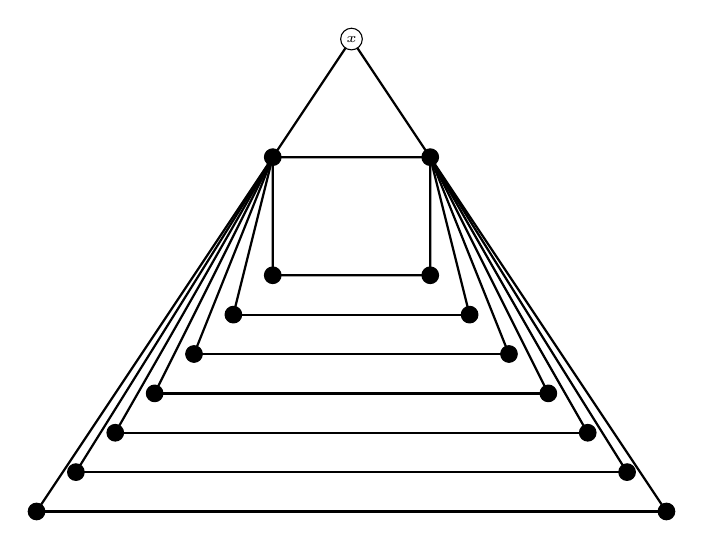
\begin{tikzpicture}[scale = 10]
\tikzstyle{VertexStyle} = []
\tikzstyle{EdgeStyle} = []
\tikzstyle{labeledStyle}=[shape = circle, minimum size = 6pt, inner sep = 1.2pt, draw]
\tikzstyle{unlabeledStyle}=[shape = circle, minimum size = 6pt, inner sep = 1.2pt, draw, fill]
\Vertex[style = labeledStyle, x = 0.700, y = 0.900, L = \tiny {$x$}]{v0}
\Vertex[style = unlabeledStyle, x = 0.600, y = 0.750, L = \tiny {}]{v1}
\Vertex[style = unlabeledStyle, x = 0.800, y = 0.750, L = \tiny {}]{v2}
\Vertex[style = unlabeledStyle, x = 0.300, y = 0.300, L = \tiny {}]{v3}
\Vertex[style = unlabeledStyle, x = 1.100, y = 0.300, L = \tiny {}]{v4}
\Vertex[style = unlabeledStyle, x = 0.600, y = 0.600, L = \tiny {}]{v5}
\Vertex[style = unlabeledStyle, x = 0.800, y = 0.600, L = \tiny {}]{v6}
\Vertex[style = unlabeledStyle, x = 0.550, y = 0.550, L = \tiny {}]{v7}
\Vertex[style = unlabeledStyle, x = 0.850, y = 0.550, L = \tiny {}]{v8}
\Vertex[style = unlabeledStyle, x = 0.500, y = 0.500, L = \tiny {}]{v9}
\Vertex[style = unlabeledStyle, x = 0.900, y = 0.500, L = \tiny {}]{v10}
\Vertex[style = unlabeledStyle, x = 0.450, y = 0.450, L = \tiny {}]{v11}
\Vertex[style = unlabeledStyle, x = 0.950, y = 0.450, L = \tiny {}]{v12}
\Vertex[style = unlabeledStyle, x = 0.400, y = 0.400, L = \tiny {}]{v13}
\Vertex[style = unlabeledStyle, x = 1.000, y = 0.400, L = \tiny {}]{v14}
\Vertex[style = unlabeledStyle, x = 0.350, y = 0.350, L = \tiny {}]{v15}
\Vertex[style = unlabeledStyle, x = 1.050, y = 0.350, L = \tiny {}]{v16}
\Edge[label = \tiny {}, labelstyle={auto=right, fill=none}](v1)(v0)
\Edge[label = \tiny {}, labelstyle={auto=right, fill=none}](v1)(v2)
\Edge[label = \tiny {}, labelstyle={auto=right, fill=none}](v1)(v3)
\Edge[label = \tiny {}, labelstyle={auto=right, fill=none}](v1)(v5)
\Edge[label = \tiny {}, labelstyle={auto=right, fill=none}](v1)(v7)
\Edge[label = \tiny {}, labelstyle={auto=right, fill=none}](v1)(v9)
\Edge[label = \tiny {}, labelstyle={auto=right, fill=none}](v1)(v11)
\Edge[label = \tiny {}, labelstyle={auto=right, fill=none}](v1)(v13)
\Edge[label = \tiny {}, labelstyle={auto=right, fill=none}](v1)(v15)
\Edge[label = \tiny {}, labelstyle={auto=right, fill=none}](v2)(v0)
\Edge[label = \tiny {}, labelstyle={auto=right, fill=none}](v2)(v4)
\Edge[label = \tiny {}, labelstyle={auto=right, fill=none}](v2)(v6)
\Edge[label = \tiny {}, labelstyle={auto=right, fill=none}](v2)(v8)
\Edge[label = \tiny {}, labelstyle={auto=right, fill=none}](v2)(v10)
\Edge[label = \tiny {}, labelstyle={auto=right, fill=none}](v2)(v12)
\Edge[label = \tiny {}, labelstyle={auto=right, fill=none}](v2)(v14)
\Edge[label = \tiny {}, labelstyle={auto=right, fill=none}](v2)(v16)
\Edge[label = \tiny {}, labelstyle={auto=right, fill=none}](v4)(v3)
\Edge[label = \tiny {}, labelstyle={auto=right, fill=none}](v6)(v5)
\Edge[label = \tiny {}, labelstyle={auto=right, fill=none}](v8)(v7)
\Edge[label = \tiny {}, labelstyle={auto=right, fill=none}](v10)(v9)
\Edge[label = \tiny {}, labelstyle={auto=right, fill=none}](v12)(v11)
\Edge[label = \tiny {}, labelstyle={auto=right, fill=none}](v14)(v13)
\Edge[label = \tiny {}, labelstyle={auto=right, fill=none}](v16)(v15)
\end{tikzpicture}
\caption{A graph $Q$ where $\gamma_r(Q - x) > \gamma_r(Q)$ for all $r \ge 3$.}
\label{fig:NotMonotone}
\end{figure}


For $r\in \IN \cup \set{\infty}$, put
\[\tilde{\gamma}(Q) \DefinedAs \max_{H \subseteq Q} \gamma_r(H).\]

\begin{conj}\label{KingEdwardsReplacement}
If $Q$ is any graph, then $\chi_f(Q) \le \tilde{\gamma}_\infty(Q)$.
\end{conj}

\begin{conj}\label{SuperDuperDuperLocalReed}
If $Q$ is a line graph, then $\chi(Q) \le \ceil{\tilde{\gamma}_\infty(Q)}$.
\end{conj}

\begin{thm}
Conjecture \ref{SuperDuperDuperLocalReed} follows from Conjecture \ref{KingEdwardsReplacement} and the Goldberg-Seymour Conjecture.
\end{thm}
\begin{proof}
Assume that Conjecture \ref{KingEdwardsReplacement} and the Goldberg-Seymour Conjecture are true and Conjecture \ref{SuperDuperDuperLocalReed} is false. 
Let $Q$ be a counterexample, say $Q = L(G)$.   
Then $\ceil{\tilde{\gamma}_\infty(Q)} < \chi(Q) \le \Delta(G) + 1 \le \omega(Q) + 1$.  So, $\ceil{\tilde{\gamma}_\infty(Q)} = \omega(Q)$ and hence
$Q$ is complete.  But that is impossible since $\omega(Q) = \ceil{\tilde{\gamma}_\infty(Q)} < \chi(Q)$.  \textcolor{red}{TODO: simplify me.}
\end{prof}

We prove the next bound in the sequence.
\begin{thm}\label{SuperDuperLocalReed}
If $Q$ is a line graph, then $\chi(Q) \le \ceil{\tilde{\gamma}_3(Q)}$.
\end{thm}

\begin{lem}\label{SuperDuperLocalReedHelper}
Let $Q = L(G)$ where $G$ is a critical graph. If $G$ is not a thickened cycle, then $\chi(Q) \le \ceil{\gamma_3(Q)}$.
\end{lem}
\begin{proof}
Suppose $G$ is not a thickened cycle. For $uv\in E(G)$, put 
\[f(uv) \DefinedAs \max\{d_G(u)+\frac12(d_G(v)-\mu(uv)),d_G(v)+\frac12(d_G(u)-\mu(uv)\}.\]
For $uv \in E(G)$, we have
\begin{align*}
f(uv) &= \frac{d_G(u) + d_G(v) - \mu(uv) + \max\set{d_G(u), d_G(v)}}{2}\\
&\le \frac{d_Q(uv) + \omega(uv) + 1}{2}.
\end{align*}
Since $G$ is critical, we have $\card{N(v)} \ge 2$ for all $v \in V(G)$.  
Since $G$ is not a thickened cycle, we may choose $x\in V(G)$ and $S\subseteq N(x)$ with $|S| = 3$ such that $x$ and $S$ achieve maximality in the definition of $d_{claw}(G)$. 
Say $S = \set{v_1, v_2, v_3}$.  Then
\begin{align*}
\ceil{\frac43\dclaw{G}} &= \ceil{\parens{\frac43}\parens{\frac14}\parens{d_G(x)+\sum_{i \in \irange{3}} d_G(v_i)}} \\
&\le \ceil{\frac13\sum_{i \in \irange{3}} d_G(v_i) + \frac12(d_G(x) - \mu(xv_i))}\\
&\le \ceil{\frac13\sum_{i \in \irange{3}} f(xv_i)}\\
&\le \ceil{\frac13\sum_{i \in \irange{3}} \frac{d_Q(xv_i) + \omega(xv_i) + 1}{2}}\\
&\le \ceil{\gamma_3(Q)}.
\end{align*}
By Theorem \ref{EasyBound2}, we have
\begin{equation}\label{EasyBoundEquation}
\chi(Q) \le \max\set{\Delta(G) + 1, \ceil{\gamma_3(Q)}}.
\end{equation}

Let $M \subseteq V(Q)$ be a maximum clique in $Q$.  
Then $\card{M} \ge 3$, so we can choose $X \subseteq M$ with $\card{X} = 3$ maximizing
\[\frac{1}{3}\sum_{v \in X} \frac{d(v) + \omega(v) + 1}{2}.\]
We have
\begin{align*}
\gamma_3(Q) &\ge \frac{1}{3}\sum_{v \in X} \frac{d(v) + \omega(v) + 1}{2}\\
&\ge \frac{1}{\card{M}}\sum_{v \in M} \frac{d(v) + \omega(v) + 1}{2}\\
&\ge \omega(Q) + \sum_{v \in M} \frac{d(v) + 1 - \omega(v)}{2}.
\end{align*}
If $V(Q) = M$, then $\ceil{\gamma_3(Q)} = \omega(Q) = \Delta(Q) = \chi(Q)$, as desired.
Otherwise, some $v \in M$ has $d(v) \ge \omega(Q)$ and hence $\ceil{\gamma_3(Q)} \ge \omega(Q) + 1 \ge \Delta(Q) + 1$.  Using 
\eqref{EasyBoundEquation}, this gives $\chi(Q) \le \ceil{\gamma_3(Q)}$.
\end{proof}

\begin{proof}[Proof of Theorem \ref{SuperDuperLocalReed}]
Suppose Theorem \ref{SuperDuperLocalReed} is false, and choose a counterexample $Q$ minimizing $\card{Q}$.
Say $Q = L(G)$.  Minimality of $\card{Q}$ and monotonicity of $\tilde{\gamma}_3$ imply that $G$ is critical.  So Lemma \ref{SuperDuperLocalReedHelper} gives
a contradiction unless $G$ is a thickened cycle.  \textcolor{red}{We should be able to finish easily, for example if King and Edwards conjecture is true 
(that $\gamma_\infty(Q)$ is an upper bound on fractional chromatic number), then since $G$ is a circular-interval graph, it has the round-up property and so
$\chi(Q) \le \ceil{\gamma_\infty(Q)} \le \gamma_3(Q)$.  But it should be simpler than that, we can compute the chromatic number directly.}
\end{proof}  
\section{Properties of long vertices}
For a path $Q$, recall that $\ell(Q)$ denotes the length of $Q$.
For $x,y \in V(Q)$, let $xQy$ denote the subpath of $Q$ with
endvertices $x$ and $y$, and let $d_Q(x,y) = \ell(xQy)$, i.e., the distance
from $x$ to $y$ along $Q$.

\begin{lem}\label{TauEscape}
Let $G$ be a critical graph with $\chi'(G) = k+1$ for some integer $k \ge \Delta(G) + 1$.
Let $\vph$ be a $k$-edge-coloring of $G-v_0v_1$. Choose $\alpha \in \vphn(v_0)$
and $\beta \in \vphn(v_1)$ and let $C = P_{v_1}(\alpha, \beta) + v_0v_1$.  If
$\tau \in \vphn(x)$ for some $x \in V(C)$ and there is a $\tau$-colored edge
from $y \in V(C)$ to $w \in V(G) \setminus V(C)$, then $C$ has a subpath $Q$
with long endpoints $z_1,z_2$ such that $x \in V(Q)$, $y \not \in V(Q-z_1-z_2)$
and the distance from $x$ to $z_i$ along $Q$ is odd for each $i \in \irange{2}$. 
Moreover, for each $i \in \irange{2}$, there are no $\tau$-colored edges
between $z_i$ and its neighbors along $C$.
\end{lem}
\begin{proof}
Let $G$, $\alpha$, $\beta$, $\tau$, $x$, and $y$ be as in the statement of the
lemma.  Choose $z_1$ (resp. $z_2$) to be the first vertex at an odd distance
from $x$ along $C$ in the clockwise (resp. counterclockwise) direction with no
incident $\tau$-colored edge parallel to some edge of $C$.  
Let $Q$ be the subpath of $C$ with endpoints $z_1$ and $z_2$ that contains $x$.
By the choice of $z_1$ each vertex $w$ between $x$ and $z_1$ with $d_Q(xw)$ odd
has a $\tau$-colored edge parallel to some edge of $C$.  The presence of these
edges implies the same for each $w$ for which $d_Q(xw)$ is even.  By the proof
of the Parallel Edge Lemma, $z_1$ must be long, since otherwise it would have an
incident $\tau$-colored edge parallel to some edge of $C$.  The same argument
applies to $z_2$.
%By rotating the $\alpha,\beta$ coloring, we can assume that $x=v_0$.
%By the Parallel Edge Lemma, we must not reach $y$ before we reach $z_1$ (resp.
%$z_2$).
%each vertex between $x$ and $z_1$ (exclusive)
%must be incident to a $\tau$-colored edge that is parallel to some edge of $C$.
%The same is true for each vertex between $x$ and $z_2$, as shown by making the
%same argument going around the cycle in the other direction.
%FILL THIS SPACE WITH PROOF.
%
%TODO: EXPLAIN WHY $y\notin\{z_1,z_2\}$ (OR CHANGE STATEMENT).
\end{proof}

\section{Thin graphs}
\label{sec:thin}
Let $G$ be a critical graph with $\chi'(G) = k+1$ for some integer $k \ge \Delta(G) + 1$.
For vertices $x \in V(G)$ and $S \subseteq V(G) \setminus \set{x}$, we say that $x$ is \emph{$S$-short} if 
every Vizing fan $F$ rooted at $x$ with $S \subseteq V(F)$, has $|F| \le 3$ (with respect to any $k$-edge-coloring of $G-xy$).
Otherwise, $x$ is \emph{$S$-long}.  For brevity, when $S = \set{y}$, we may write $y$-short instead of $\set{y}$-short.
It is worth noting that in Lemma~\ref{SpecialPath} we can weaken the hypothesis
that $v_i$ is short for all odd $i$ to require only that $v_i$ is
$v_{i-1}$-short for all odd $i$, since this is what we use in the proof.  

A graph $G$ is \emph{$k$-thin} if $\mu(G) < 2k - d(x) - d(y)$ for all
long $x,y \in V(G)$.  In the proof of Theorem~\ref{mainhelper}, we will show that
every counterexample to the $\frac56$-Conjecture must be $k$-thin.

\begin{lem}\label{NonSpecialsInThinAreAtEvenDistance}
Let $G$ be a $k$-thin, critical graph with $\chi'(G) = k+1$ for some integer $k \ge \Delta(G) + 1$.
Let $\vph$ be a $k$-edge-coloring of $G-v_0v_1$. Choose $\alpha \in \vphn(v_0)$
and $\beta \in \vphn(v_1)$ and let $C = P_{v_1}(\alpha, \beta) + v_0v_1$.
Let $Q$ be a subpath of $C$ with long end vertices.  If all internal vertices
of $Q$ are short and $2 \le \ell(Q) \le \ell(C) - 2$, then $\ell(Q)$ is even.
\end{lem}
\begin{proof}
Suppose to the contrary that we have a subpath $Q$ of $C$ with end vertices
long, all internal vertices short, $2\le \ell(Q) \le \ell(C) - 2$,
and $\ell(Q)$ odd.  Let $x$ and $y$ be the end vertices of $Q$.
Say $C = v_1v_2\cdots v_rv_0v_1$.  By rotating the $\alpha,\beta$ coloring of
$C$, we may assume that $x = v_0$ and $y = v_a$, where $a \ge 3$ is odd.

We now apply Lemma \ref{SpecialPath} twice, to show that $\mu(v_1v_2) \ge 2k -
d(v_0) - d(v_a)$, which contradicts that $G$ is $k$-thin.  More specifically,
assume that the edges $v_0v_1,v_1v_2,\ldots$ go clockwise around $C$.  We apply
Lemma~\ref{SpecialPath} once going clockwise starting from $v_0$ and once going
counterclockwise starting from $v_a$.  The first application implies that every
color in $\vphn(v_0)$ appears on some edge parallel to $v_1v_2$; the second
implies the same for every color in $\vphn(v_a)$.  Since $|\vphn(v_i)|=k-d(v_i)$
for each $i\in\{0,a\}$ and $\vphn(v_0)\cap \vphn(v_a)=\emptyset$, the conclusion
follows.
\end{proof}

\begin{lem}\label{ThreeNonSpecialOnCycle}
Let $G$ be a $k$-thin, critical graph with $\chi'(G) = k+1$ for some integer $k
\ge \Delta(G) + 1$.  Let $\vph$ be a $k$-edge-coloring of $G-v_0v_1$. Suppose
$\alpha \in \vphn(v_0)$ and $\beta \in \vphn(v_1)$ and let $C = P_{v_1}(\alpha,
\beta) + v_0v_1$.  If $C$ contains exactly 3 long vertices, then $C = xyAzBx$
where $A$ and $B$ are paths of even length and $x,y,z$ are all long.  Moreover,
$x$ is $y$-long and $y$ is $x$-long.
\end{lem}
\begin{proof}
Let $G$ be a graph satisfying the hypotheses, and let $x$, $y$, $z$ be the
three long vertices.
The three subpaths of $C$ with endpoints $x$,
$y$, and $z$ either (i) all have odd length or (ii) include two paths of even
length and one of odd length.  
First assume that $\ell(C)\ge 5$.  
%Since $\ell(C)\ge 5$, 
If we are in (i), then the longest of these three subpaths
violates Lemma~\ref{NonSpecialsInThinAreAtEvenDistance}; so we are in (ii), and
also the path of odd length is simply an edge.  This proves the first statement.
For the second statement, assume to the contrary that $x$ is $y$-short.
By rotating the $\alpha,\beta$ coloring, we can assume that $y=v_0$ and $x=v_1$.
As in the previous lemma, we use Lemma~\ref{SpecialPath} (and the comment in the
first paragraph of Section~\ref{sec:thin}) to conclude that $\mu(v_1v_2)\ge
2k-d(v_0)-d(z)$.  As above, this contradicts that $G$ is $k$-thin; this
contradiction proves the second statement.
\end{proof}

\begin{lem}\label{ConsecutiveNonSpecials}
Let $G$ be a non-elementary, $k$-thin, critical graph with $\chi'(G) = k+1$ for
some integer $k \ge \Delta(G) + 1$.  Choose $(T, v_0v_1, \vph) \in \T(G)$. If
$\alpha \in \vphn(v_0)$ and $\beta \in \vphn(v_1)$, then $P_{v_1}(\alpha,
\beta) + v_0v_1$ contains consecutive long vertices.
\end{lem}
\begin{proof}
Let $C = P_{v_1}(\alpha, \beta) + v_0v_1$.  By Lemma \ref{FreeColorsLemma},
there is $x \in V(C)$ and $\tau \in \vphn(x)$ such that there is a
$\tau$-colored edge from $y \in V(C)$ to $w \in V(T) \setminus V(C)$.
Lemma \ref{TauEscape} implies that $C$ has a subpath $Q$ with $x \in V(Q)$
 and long endpoints $z_1,z_2$ such that the distance from $x$ to
$z_i$ along $Q$ is odd for each $i \in \irange{2}$.  
Let $Q'$ be the subpath of $C$ with endpoints $z_1$ and $z_2$ that does not contain
$x$. Since $C$ is an odd cycle, $\ell(Q')$ is odd.  Let $Q^*$ be a minimum
length subpath of $Q'$ with long ends.  Now $\ell(Q^*) = 1$ by Lemma
\ref{NonSpecialsInThinAreAtEvenDistance}, as desired.
\end{proof}

\begin{lem}\label{MasterHelper}
Let $G$ be a non-elementary, $k$-thin, critical graph with $\chi'(G) = k+1$ for
some integer $k \ge \Delta(G) + 1$.  If $(T, v_0v_1, \vph) \in \T(G)$ and
$\nu(T) \le 3$, then $T$ contains long vertices $z_1,z_2,z_3$ such that either 
\begin{enumerate}
\item $z_1$ is $\set{z_2,z_3}$-long and $z_2$ is $z_1$-long; or
%\item $z_i$ is $z_{3-i}$-long and $z_{i+1}$ is $z_{4-i}$-long for $i \in \irange{2}$.
\item $z_i$ is $z_j$-long and $z_j$ is $z_i$-long for each %unordered pair
$(i,j)\in\{(1,2),(2,3)\}$.
\end{enumerate}
\end{lem}
\begin{proof}
Choose $\alpha \in \vphn(v_0)$ and $\beta \in \vphn(v_1)$ so that
$P_{v_1}(\alpha, \beta)$ contains as many long vertices as possible;
let $C=P_{v_1}(\alpha,\beta)+v_0v_1$.
By Lemma \ref{FreeColorsLemma}, there is $x \in V(C)$ and $\tau \in \vphn(x)$
such that there is a $\tau$-colored edge from $y \in V(C)$ to $w \in V(T)
\setminus V(C)$.  By Lemma~\ref{ConsecutiveNonSpecials}, $C$ has at least two
long vertices.

First suppose that $C$ contains only 2 long vertices, $z_1$ and $z_2$.  By
Lemma \ref{ConsecutiveNonSpecials}, $z_1$ and $z_2$ are consecutive on $C$.
Lemma \ref{TauEscape} implies that $C$ has a subpath $Q$ 
with endpoints $z_1,z_2$ such that $x \in V(Q)$ and $y \not \in V(Q-z_1-z_2)$ 
and for each $i \in \irange{2}$ 
there are no $\tau$-colored edges between $z_i$ and its neighbors on $C$.
%
By rotating the $\alpha,\beta$ coloring of $C$, we can assume that $x = v_0$ and
$\alpha,\tau\in \vphn(v_0)$ and $\beta\in\vphn(v_1)$. 
Note that $P_{v_1}(\tau,\beta)$ must end at $v_0$ (since otherwise we can
recolor the Kempe chain and color $v_0v_1$ with $\tau$).  
Let $C' = P_{v_1}(\tau, \beta) + v_0v_1$.  Note that $C'$ must include $v_1Qz_1$
and also $v_0Qz_2$ (the $\beta$-colored edges are present by definition and the
$\tau$-colored edges are present by the Parallel Edge Lemma).  Thus, $z_1,z_2\in
V(C')$.  Since $z_1$ and $z_2$ are not consecutive on $C'$
and $C'$ contains no other long vertices by the maximality condition on $C$,
Lemma \ref{ConsecutiveNonSpecials} gives a contradiction.

So instead $C$ contains exactly 3 long vertices, $z_1$, $z_2$, and $z_3$.  By Lemma
\ref{ThreeNonSpecialOnCycle}, $C = z_1z_2Az_3Bz_1$ where $A$ and $B$ are paths
of even length.  Also, $z_1$ is $z_2$-long and $z_2$ is $z_1$-long.  

By Lemma \ref{TauEscape}, $C$ has a subpath $Q$ 
with endpoints $z_1,z_3$ and with $x \in V(Q)$ and $y \not
\in V(Q-z_1-z_3)$ 
such that there are no $\tau$-colored edges
between $z_i$ and its neighbors along $C$ for each $i \in \set{1,3}$ (it could
happen that $z_3$ has a $\tau$-colored edge parallel to an edge of $C$,
so the endpoints of $Q$ are $z_1, z_2$, but now we get a contradiction
as in the previous case, by letting $C'=P_{v_1}(\tau,\beta)+v_0v_1$).  By
rotating the $\alpha,\beta$ coloring of $C$, we
may assume that $x = v_0$.  Again, let $C' = P_{v_1}(\tau, \beta) + v_0v_1$.  We
know that $C'$ contains $z_1$ and $z_3$ and that $z_1$ and $z_2$ are not
consecutive on $C'$.  Note also that all long vertices in $V(C')$ must be among
$z_1,z_2,z_3$, since otherwise $\nu(T)\ge 4$, contradicting our hypothesis.
So by Lemma~\ref{ConsecutiveNonSpecials}, either $z_1$ and
$z_3$ are consecutive on $C'$ or $z_2$ and $z_3$ are consecutive on $C'$.

Suppose that $z_2$ and $z_3$ are consecutive on $C'$, and thus connected by a
$\tau$-colored edge.  Now applying Lemma \ref{ThreeNonSpecialOnCycle} shows that $z_2$
is $z_3$-long and $z_3$ is $z_2$-long, so we satisfy (2) in the conclusion of
the lemma (by swapping the names of $z_1$ and $z_2$).

So instead $z_1$ and $z_3$ must be consecutive on $C'$, and thus connected by a
$\tau$-colored edge.  If $z_1 = v_1$, then we have a fan with an
$\alpha$-colored edge from $z_1$ to $z_2$ and a $\tau$-colored edge from $z_1$
to $z_3$, so $z_1$ is $\set{z_2,z_3}$-long. 

Now assume that $z_1\ne v_1$.
Let $z_1'$ be the predecessor of $z_1$ on the path from $v_0$ (through $v_1$) to
$z_1$.  We can shift the coloring so that $z_1'z_1$ is uncolored and $z_1z_2$
is colored $\alpha$ (as in the proof of the Parallel Edge Lemma).  In fact, 
we can shift either the $\alpha,\beta$ edges or the $\tau,\beta$ edges.  This
gives the options that either $\alpha\in \vphn(z_1')$ or $\tau\in \vphn(z_1')$,
whichever we prefer.  Suppose we shift the $\tau,\beta$ edges.
Now choose $\gamma\in \vphn(z_1')-\alpha-\tau$.  Consider
the $\gamma$-colored edge $e$ incident to $z_1$.  If $e$ goes to $z_2$, then we
$z_1$ is $\{z_2,z_3\}$-long, by colors $\gamma$ and $\tau$; so we satisfy (1) in
the conclusion of the lemma.
If instead $e$ goes to $z_3$, then instead of shifting the $\tau,\beta$ edges we
shift the $\alpha,\beta$ edges; note that this recoloring preserves the fact
that $\gamma$ is missing at $z_1'$.  Now again $z_1$ is $\{z_2,z_3\}$-long, this
time by colors $\alpha$ and $\gamma$; so we again satisfy (1) in the conclusion
of the lemma.

Finally, assume that the $\gamma$-colored edge incident to $z_1$ goes to some
vertex other than $z_2$ and $z_3$.  Now let $C''=P_{z_1}(\gamma,\beta)+z_1z_1'$.
Since $V(C'')\subseteq V(T)$, Lemmas~\ref{ConsecutiveNonSpecials} and
\ref{ThreeNonSpecialOnCycle} imply that $z_2$ and $z_3$ are
adjacent on $C''$ and furthermore $z_2$ is $z_3$-long and $z_3$ is $z_2$-long;
thus, we satisfy (2) in the conclusion of the lemma.
%can win by shifting the $\tau,\gamma$ edges.  Similarly, if $e$ goes to $z_3$, then
%we can win by shifting the $\alpha,\gamma$ edges.  
%The question is why do we know that e goes to either z_2 or z_3?
%When $z_1 \ne v_1$, we get the same thing, but have to shift the coloring over
%to $z_1$ like in the proof of Lemma \ref{SpecialPath} using another missing
%color $\gamma$ at $z_1$.
\end{proof}

We need the following result from~\cite{rabern2011strengthening}, which we use
to handle the case when $G$ is not $k$-thin.

\begin{thm}[\cite{rabern2011strengthening}]\label{CriticalMuBound}
If $Q$ is the line graph of a graph $G$ and $Q$ is vertex critical, then
\[\chi(Q) \leq \max\left\{\omega(Q), \Delta(Q) + 1 - \frac{\mu(G) - 1}{2}\right\}.\]
\end{thm}

Now we prove the main result of this section.

\begin{thm}
If $Q$ is the line graph of $G$, then
\[\chi(Q) \le \max\set{\W(Q), \Delta(G) + 1, \frac{5\Delta(Q) + 8}{6}}.\]
\label{mainhelper}
\end{thm}
\begin{proof}
Suppose the theorem is false and choose a counterexample minimizing $\card{Q}$.
Let $k = \max\set{\W(Q), \Delta(G) + 1, \frac{5\Delta(Q) + 8}{6}}$. Say $Q =
L(G)$ for a graph $G$. The minimality of $Q$ implies that
$G$ is critical and $\chi(Q) = k+1$, for some $k \ge \Delta(G) + 1$.

The heart of the proof is Claim~1, which roughly says that if $x$ is long, then
$d(x)<\frac34\Delta(G)$. Moreover, we can improve this bound further if $x$ is
the root of a long fan $F$ such that either (i) $F$ has length more than 3 or (ii)
some of the other vertices in $F$ have degree less than $\Delta(G)$.  The claims
thereafter are all essentially applications of Claim~1.
\bigskip

\claim{1}{Let $F$ be a fan rooted at $x$ with respect to a $k$-edge-coloring of
$G - xy$.  If $S\subseteq V(F)-x$ and $|S| \ge 3$, then
\[d(x) \le \frac1{5|S|-11}\parens{2|S|-12 + \sum_{v \in S} d(v)}.\]
In particular, if $|S|=3$, then $d(x) \le \frac1{4}\parens{-6 + \sum_{v \in S}
d(v)}.$}
\begin{claimproof}
Since $F$ is elementary, we have
\[2 + k-d(x) + \sum_{v \in S} k - d(v) \le k,\]
so
\[2 + |S|k \le d(x) + \sum_{v \in S} d(v).\]
Using $k \ge \frac56(\Delta(Q) + 1) - \frac13 \ge \frac56(d(x) + d(v) - \mu(xv))
- \frac13$ for each $v
\in S$, we get
\[2 + \sum_{v \in S}\parens{\frac56(d(x) + d(v) - \mu(xv)) -\frac13} \le d(x) +
\sum_{v \in S} d(v),\]
so multiplying by 6 and rearranging terms gives
\[12 + \parens{5|S| - 6}d(x) - 2|S| \le \sum_{v \in S} 5\mu(xv) + \sum_{v \in S} d(v).\]
Now $\sum_{v \in S} \mu(xv) \le d(x)$, so this implies
\[12 + \parens{5|S| - 11}d(x) - 2|S| \le \sum_{v \in S} d(v).\]
Solving for $d(x)$ gives
\[d(x) \le \frac1{5|S|-11}\parens{2|S|-12 + \sum_{v \in S} d(v)},\]
and when $|S| = 3$, we get
$d(x) \le \frac14\parens{-6 + \sum_{v \in S} d(v)}.$
\end{claimproof}
\bigskip

\claim{2}{If $x \in V(G)$ is long, then $d(x) \le \frac34\Delta(G) - 1$.}

\begin{claimproof}
This is immediate from Claim 1, since $d(v)\le \Delta(G)$ for all $v\in S$.
\end{claimproof}
\bigskip

\claim{3}{If $x_1x_2 \in E(G)$ such that $x_1$ is $x_2$-long and $x_2$ is
$x_1$-long, % for all $i \in \irange{2}$, 
then
\[d(x_i) \le \frac23\Delta(G) -2 \text{ for all $i \in \irange{2}$.}\]}

\begin{claimproof}
By Claim 1, for each $i \in \irange{2}$,
\[d(x_i) \le \frac14\parens{-6 + \sum_{v \in S} d(v)} \le \frac14\parens{-6 + d(x_{3-i}) + 2\Delta(G)},\]
Substituting the bound on $d(x_{3-i})$ into that on $d(x_i)$ and simplifying
gives for each $i \in \irange{2}$,
\[d(x_i) \le -2 + \frac23\Delta(G).\]
\end{claimproof}

\bigskip

\claim{4}{If $x_1x_2, x_1x_3 \in E(G)$ such that $x_1$ is $\set{x_2,x_3}$-long, $x_2$ is $x_1$-long and $x_3$ is long, then 
\[d(x_1) \le -\frac85 + \frac35\Delta(G),\]
\[d(x_2) \le -\frac75 + \frac{13}{20}\Delta(G).\]}

\begin{claimproof}
By Claim 1, we have
\[d(x_1) \le \frac14\parens{-6 + \sum_{v \in S} d(v)} \le \frac14\parens{-6 + d(x_2) + d(x_3) + \Delta(G)},\]
\[d(x_2) \le \frac14\parens{-6 + \sum_{v \in S} d(v)} \le \frac14\parens{-6 + d(x_1) + 2\Delta(G)}.\]
By the same calculation as in Claim~3, these together imply
\[d(x_1) \le -2 + \frac25\Delta(G) + \frac{4}{15}d(x_3).\]
Since $x_3$ is long, using Claim 2, we get
%\[d(x_1) \le -\frac85 + \frac35\Delta(G),\]
\[d(x_1) \le -\frac{34}{15} + \frac35\Delta(G),\]
and hence
%\[d(x_2) \le -\frac75 + \frac{13}{20}\Delta(G).\]
\[d(x_2) \le -\frac{61}{15} + \frac{13}{20}\Delta(G).\]
\end{claimproof}
\bigskip

\claim{5}{The theorem is true.}

\begin{claimproof}
Let $(T, v_0v_1, \vph) \in \T(G)$. By Lemma \ref{MasterHelper}, one of the following holds:
\begin{enumerate}
\item $G$ is elementary; or
\item $G$ is not $k$-thin; or
\item $\nu(T) = 3$ and $V(T)$ contains vertices $x_1,x_2,x_3$ such that $x_1$
is $x_2$-long, $x_2$ is $x_1$-long, $x_2$ is $x_3$-long, and $x_3$ is $x_2$-long; or
\item $\nu(T) = 3$ and $V(T)$ contains vertices $x_1,x_2,x_3$ such that $x_1$ is
$\set{x_2,x_3}$-long, $x_2$ is $x_1$-long, and $x_3$ is long; or
\item $V(T)$ contains four long vertices $x_1, x_2, x_3, x_4$.
\end{enumerate}

%If (1) holds, then $k + 1 = \ceil{\chi_f(Q)} \le k$, a contradiction.
If (1) holds, then $\chi(Q) = \ceil{\chi_f(Q)}$, which contradicts our choice of
$Q$ as a counterexample.

If (2) holds, then Claim 2 implies that $\mu(G) \ge 2k - \frac32\Delta(G) + 2$. 
Now Theorem \ref{CriticalMuBound} gives
\begin{align*}
k + 1 &\le \Delta(Q)+1-\frac{2k-\frac32\Delta(G)+2}2\\
&=\Delta(Q) + 1 - k +
\frac34\Delta(G) - 1,
\end{align*}
so
\[2(k + 1) \le \Delta(Q) + 1 + \frac34\Delta(G).\]

Substituting $\Delta(G) \le k$ and solving for $k$ gives

\[k  \le \frac45\Delta(Q) - \frac45 < \frac56\Delta(Q)+\frac12 \le k,\]
which is a contradiction.

Suppose (3) holds.  
Now \[2 + \sum_{i \in \irange{3}} k - d(x_i) \le k,\]
so Claim 3 implies
\[3\parens{\frac23\Delta(G) -2} \ge 2k+2,\]
which is a contradiction, since $\Delta(G) \le k$.

Suppose (4) holds.  Now
\[2 + \sum_{i \in \irange{3}} k - d(x_i) \le k,\]
so Claims 2 and 4 give
\[ \parens{\frac35 + \frac{13}{20} + \frac34}\Delta(G)-\parens{\frac{34}{15} + \frac{16}{15} + 1}\ge 2k+2,\]
which is
\[2\Delta(G) -\frac{13}3\ge 2k+2,\]
again a contradiction, since $\Delta(G) \le k$.


So (5) must hold.  But now
\[2 + \sum_{i \in \irange{4}} k - d(x_i) \le k,\]
so using Claim 2 gives
\[4\parens{\frac34\Delta(G) - 1} \ge 3k+2,\]
a contradiction since $\Delta(G) \le k$.
\end{claimproof}

This finishes the final case of Claim~5, which proves the theorem.
\end{proof}

In the previous theorem, we showed that 
$\chi(Q) \le \max\set{\W(Q), \Delta(G) + 1, \frac{5\Delta(Q) +
8}{6}}$.  Now we show that if the maximum is attained by the second argument,
then $G$ satisfies the $\frac56$-Conjecture.
We use the following lemma, which is implicit in~\cite{rabern2011strengthening};
see the proof of Lemma~9 therein.

\begin{lem}\label{CriticalMuBoundOtherWay}
If $Q$ is the line graph of a graph $G$ and $Q$ is vertex critical, then
\[\chi(Q) \leq \max\left\{\Delta(G), \Delta(Q) + 1 + 2\mu(G) - \Delta(G)\right\}.\]
\end{lem}
%\begin{proof}
%The fan equation implies this (see the proof in strengthening Brooks paper).
%\end{proof}

\begin{cor}
If $Q$ is the line graph of a critical graph $G$ and $\chi(Q) \le \Delta(G) + 1$, then
\[\chi(Q) \le \max\set{\omega(Q), \frac{5\Delta(Q) + 8}{6}}.\]
\label{mainCorHelper}
\end{cor}
\begin{proof}
Let $k +1=\chi(Q) \le \Delta(G)+1$.  Suppose $\chi(Q) > \omega(Q)$.  Then Lemma \ref{CriticalMuBoundOtherWay} gives
\[k + 1 = \chi(Q) \le \Delta(Q) + 1 + 2\mu(G) - k,\]
so solving for $\mu(G)$ gives
\[\mu(G) \ge k - \frac{\Delta(Q)}{2}.\]
Applying Theorem \ref{CriticalMuBound} gives
\[k+1 = \chi(Q) \le \Delta(Q) + 1 - \frac{k - \frac{\Delta(Q)}{2} - 1}{2},\]
and solving for $k+1$ yields
\[\chi(Q) = k+1 \le \frac56\Delta(Q) + \frac43 = \frac{5\Delta(Q) + 8}{6}.\]
\end{proof}

Since $\omega(Q) \le \max\{\Delta(G),\W(G)\}$, Theorem~\ref{mainhelper} and
Corollary~\ref{mainCorHelper} together imply the following.

\begin{cor}
If $Q$ is the line graph of a graph $G$, then
\[\chi(Q) \le \max\set{\Delta(G),\W(G), \frac{5\Delta(Q) + 8}{6}}.\]
\label{mainCor}
\end{cor}

\section{The $\frac56$-Conjecture}
\label{sec:final}
\begin{lem}
Let $G$ be a critical, elementary graph with $\chi'(G) = k + 1$ where $k \ge \Delta(G) + 1$.  Put $Q \DefinedAs L(G)$.  
If $k = \epsilon\parens{\Delta(Q) + 1} + \beta$, then for all $x \in V(G)$,
\[\card{N(x)} = \frac{\epsilon\parens{|G| - \Delta(G) - d_G(x) - 1 + S_1 + S_2 + S_3\parens{\card{G} - 1}}}{(1-\epsilon)\Delta(G) - \epsilon d_G(x) + 1 - \beta + S_3},\]
where 
\[S_1 \DefinedAs \sum_{v \in N(x)} \Delta(Q) - d_Q(xv),\]
\[S_2 \DefinedAs 2 + \sum_{v \in V(G) \setminus N(x)} \Delta(G) - d_G(v),\]
\[S_3 \DefinedAs k - (\Delta(G) + 1).\]
\end{lem}
\begin{proof}
Since $G$ is critical and elementary, $\card{G}$ is odd and
\begin{equation}\label{eq1}
k = \frac{2(\size{G} - 1)}{\card{G} - 1}.
\end{equation}
Let $x \in V(G)$, put $M \DefinedAs \card{N(x)}$ and 
\[P \DefinedAs \sum_{v \in N(x)} d_G(v).\] 
Then
\begin{equation}\label{eq2}
2(\size{G} - 1) = \Delta(G)(|G| - M) - S_2 + P.
\end{equation}
Since 
\[\frac{2(\size{G} - 1)}{\card{G} - 1} = k = \Delta(G) + 1 + S_3,\]
using \eqref{eq2}, we get
\[P = (|G| - 1)(\Delta(G) + 1 + S_3) - \Delta(G)(|G| - M) + S_2,\]
which is
\begin{equation}\label{eq3}
P = \Delta(G)(M-1) + |G| - 1 + S_2 + S_3(|G| - 1).
\end{equation}
Also, using $k = \epsilon\parens{\Delta(Q) + 1} + \beta$, we get
\[kM = \beta M + \epsilon S_1 + \epsilon\sum_{v \in N(x)} d_G(x) + d_G(v) - \mu(xv),\]
Since $\sum_{v \in N(x)} \mu(xv) = d_G(x)$,we have
\begin{equation}\label{eq4}
kM = \beta M + \epsilon S_1 + \epsilon d_G(x)(M - 1) + \epsilon P.
\end{equation}
Plugging \eqref{eq3} into \eqref{eq4} and solving for $M$ gives
\[M= \frac{\epsilon\parens{|G| - \Delta(G) - d_G(x) - 1 + S_1 + S_2 + S_3\parens{\card{G} - 1}}}{(1-\epsilon)\Delta(G) - \epsilon d_G(x) + 1 - \beta + S_3},\]
as desired.
\end{proof}

Using $\epsilon = \frac56$, we get the following.

\begin{lem}\label{Slacked56}
Let $G$ be a critical, elementary graph with $\chi'(G) = k + 1$ where $k \ge \Delta(G) + 1$.  Put $Q \DefinedAs L(G)$. 
If $k = \frac56\parens{\Delta(Q) + 1} + \beta$, then for all $x \in V(G)$,
\[\card{N(x)} = \frac{5\parens{|G| - \Delta(G) - d_G(x) - 1 + S_1 + S_2 + S_3\parens{\card{G} - 1}}}{\Delta(G) - 5 d_G(x) + 6(1 - \beta + S_3)},\]
where 
\[S_1 \DefinedAs \sum_{v \in N(x)} \Delta(Q) - d_Q(xv),\]
\[S_2 \DefinedAs 2 + \sum_{v \in V(G) \setminus N(x)} \Delta(G) - d_G(v),\]
\[S_3 \DefinedAs k - (\Delta(G) + 1).\]
\end{lem}


\begin{lem}\label{DegreeBoundedForMiddling}
Let $G$ be a critical, elementary graph with $\chi'(G) = k + 1$ where $k \ge \Delta(G) + 1$.  Put $Q \DefinedAs L(G)$. 
If $k = \frac56\parens{\Delta(Q) + 1} + \beta$ where $\beta \ge -\frac13$, then for all $x \in V(G)$ with $\card{N(x)} \ge 3$,
\[d_G(x) \le \frac{3}{5}\Delta(G) - \frac{1}{\card{N(x)} - 2}\sum_{v \in V(G)\setminus N[x]} \Delta(G) - d_G(v).\]
If additionally, $\card{N(x)} \le \frac58\card{G}$, then
\[d_G(x) \le \frac{\card{N(x)}}{5\parens{\card{N(x)} - 2}}\Delta(G) - \frac{1}{\card{N(x)} - 2}\sum_{v \in V(G)\setminus N[x]} \Delta(G) - d_G(v).\]
\end{lem}
\begin{proof}
Say $|N(x)| = 2 + S_4$ for some $S_4 \ge 1$.  Applying Lemma \ref{Slacked56} and simplifying using $S_1 \ge 0$ and $\beta \ge -\frac13$ gives
\begin{equation}\label{longeq}
(5+5S_4)d_G(x) \le (7 + S_4)\Delta(G) - 5|G| + 21 + S_3(-5|G| + 17 + 6S_4) + 8S_4 - 5S_2.
\end{equation}
Put 
\[t \DefinedAs \sum_{v \in V(G) \setminus N[x]} \Delta(G) - d_G(v).\]
Then $S_2 = t + 2 + \Delta(G) - d_G(x)$.  Using this in \eqref{longeq}, we get
\begin{equation}\label{longeq2}
5S_4d_G(x) \le (2 + S_4)\Delta(G) - 5|G| + 11 + S_3(-5|G| + 17 + 6S_4) + 8S_4 - 5t.
\end{equation}
The desired bound follows when $S_4 \le \frac58\card{G} - 2$, since then
\[- 5|G| + 11 + S_3(-5|G| + 17 + 6S_4) + 8S_4 \le 0.\]

So, suppose $S_4 > \frac58\card{G} - 2$. Rearranging \eqref{longeq2}, we get
\begin{equation}\label{longeq3}
5S_4d_G(x) \le 3S_4\Delta(G) - 5|G| + 11 + S_3(-5|G| + 17 + 6S_4) + 8S_4 - (2S_4-2)\Delta(G) - 5t
\end{equation}
Now $S_4 = \card{N(x)} - 2 = \card{G} - 3 + S_5$, where
\[S_5 \DefinedAs S_4 + 3 - \card{G} \le 0.\]
Thus
\[-5|G| + 15 + 5S_4 +S_3(-5|G| + 15 + 5S_4) - 5S_5(1 + S_3) = 0,\]
so
\begin{equation}\label{longeq4}
5S_4d_G(x) \le 3S_4\Delta(G) - 4 + 2S_3 + (S_3 + 3)S_4 - (2S_4-2)\Delta(G) + 5S_5(1 + S_3) - 5t 
\end{equation}
If
\[-4 + 2S_3 + (S_3 + 3)S_4 - (2S_4-2)\Delta(G) + 5S_5(1 + S_3) \le 0,\]
then we have the contradiction
\[d_G(x) \le \frac{3}{5}\Delta(G) - \frac{1}{\card{N(x)} - 2}\sum_{v \in V(G)\setminus N[x]} \Delta(G) - d_G(v).\]
So, we have
\[-4 + 2S_3 + (S_3 + 3)S_4 - (2S_4-2)\Delta(G) + 5S_5(1 + S_3) > 0,\]
which is
\begin{equation}\label{MM3}
(2 + S_4)S_3 + 3S_4 > (2S_4-2)\Delta(G) + 4 - 5S_5(S_3 + 1).
\end{equation}
By Shannon's theorem $k + 1 \le \frac32\Delta(G)$, so $S_3 \le \frac{\Delta(G)}{2} - 2$. After plugging in for $S_3$ on the left side and solving for $S_4$, we get
\[S_5 + \card{G} - 3 = S_4 < \frac{6\Delta(G) - 16 + 10S_5(S_3+1)}{3\Delta(G) - 2} = 2 + \frac{5S_5(S_3 + 1) - 12}{3\Delta(G) - 2},\]
so
\[\card{G} < 5 + \frac{(10S_3 - 3\Delta(G) + 12)S_5 - 12}{3\Delta(G) - 2}.\]
Since $S_5 \le 0$, this implies $\card{G} \le 3$, unless $10S_3 - 3\Delta(G) + 12 < 0$.  So $S_3 < \frac{3}{10}\Delta(G) - \frac65$. 
Since $S_5 \le 0$, \eqref{MM3} implies
\[(2 + S_4)S_3 + 3S_4 > (2S_4-2)\Delta(G) + 4\]
Plugging in $S_3 < \frac{3}{10}\Delta(G)-\frac65$ gives
\[\card{G} - 3 \le S_4 < \frac{26\Delta(G) - 64}{17\Delta(G) - 18} < 2,\]
a contradiction.
\end{proof}

\begin{cor}\label{CriticalElementary56}
Let $G$ be a critical, elementary graph with $\chi'(G) = k + 1$ where $k \ge \Delta(G) + 1$.  Put $Q \DefinedAs L(G)$. 
If $k = \frac56\parens{\Delta(Q) + 1} + \beta$ where $\beta \ge -\frac13$, then there is at most one $x \in V(G)$ with $\card{N(x)} \ge 3$.
\end{cor}
\begin{proof}
Since $G$ is critical and elementary, $\card{G}$ is odd and
\[\frac{2(\size{G} - 1)}{\card{G} - 1} = k \ge \Delta(G) + 1,\]
so
\[2\size{G} \ge \Delta(G)\card{G} + \card{G} - \Delta(G) + 1.\]
In particular,
\[\sum_{v \in V(G)} \Delta(G) - d_G(v) \le \Delta(G) - 1 - \card{G}.\]
By Lemma \ref{DegreeBoundedForMiddling}, every $x \in V(G)$ with $\card{N(x)} \ge 3$ has $d_G(x) \le \frac35\Delta(G)$, so there are at most two such $x$ since
$\frac25 + \frac25 + \frac25 > 1$.  Suppose there are $x_1, x_2$ with $\card{N(x_1)} \ge \card{N(x_2)} \ge 3$.

Let $z \in V(G)$ with $d_G(z) = \Delta(G)$.  Then, by Lemma \ref{DegreeBoundedForMiddling}, $\card{N(z)} = 2$, so $\mu(G) \ge \frac12\Delta(G)$.
By Theorem \ref{CriticalMuBound}, $\mu(G) < \frac13(\Delta(Q) + 1)$.  We conclude
\begin{equation}
\Delta(G) < \frac23(\Delta(Q) + 1).\label{DeltaGQUpperBound}
\end{equation}

First, suppose $x_1 \adj x_2$.  Since $Q$ is vertex-critical, 
\begin{align*}
k &\le d_Q(x_1x_2)\\
&=d_G(x_1) + d_G(x_2) - \mu(x_1x_2) - 1\\
&\le \frac65\Delta(G) - \mu(x_1x_2) - 1,
\end{align*}
So, $\Delta(G) >\frac56k$.  By \eqref{DeltaGQUpperBound},
\[\frac56k < \Delta(G) < \frac23(\Delta(Q) + 1),\]
and hence $k < \frac45(\Delta(Q) + 1)$, a contradiction.  

So, $x_1 \nonadj x_2$. Now suppose $\card{N(x_2)} \le \frac58\card{G}$.  Since $x_1 \nonadj x_2$, Lemma \ref{DegreeBoundedForMiddling} gives
\[d_G(x_2) \le \frac35\Delta(G) - (\Delta(G) - d_G(x_1)) \le \frac15\Delta(G),\]
a contradiction since $\frac45 + \frac25 > 1$. 

So, $\card{N(x_i)} > \frac58\card{G}$ for $i \in \irange{2}$.  In particular, there is $y \in N(x_1) \cap N(x_2)$.  Since $\card{N(y)} = 2$, by symmetry
we may assume $\mu(x_1y) \ge \frac12 d_G(y)$.  Hence, using \eqref{DeltaGQUpperBound},
\begin{align*}
k &\le d_Q(x_1y) \\
&= d_G(x_1) + d_G(y) - \mu(x_1y) < d_G(x_1) + \frac12d_G(y) \\
&\le \frac{11}{10}\Delta(G) \\
&< \frac{11}{15}(\Delta(Q) + 1),
\end{align*}
a contradiction.
\end{proof}

\begin{thm}
If $Q$ a line graph, then
\[\chi(Q)\le \max\set{\omega(Q),\ceil{\frac{5\Delta(Q)+3}{6}}}.\]
\end{thm}
\begin{proof}
Suppose the theorem is false and choose a counterexample $Q$ minimizing $\card{Q}$.  Then $Q = L(G)$ for a critical graph $G$.  Say $\chi(Q) = \chi'(G) = k + 1$.  Then
$k = \max\set{\omega(Q),\ceil{\frac{5\Delta(Q)+3}{6}}}$ by minimality of $\card{Q}$.  By Corollary \ref{mainCor},
\[k+1 \le \max\set{\ceil{\chi_f(Q)}, \ceil{\frac{5\Delta(Q)+3}{6}}},\]
so
\[\ceil{\chi_f(Q)} = \ceil{\frac{5\Delta(Q)+3}{6}} + 1 = \chi(Q).\]
Therefore $G$ is elementary and $k = \frac56\parens{\Delta(Q) + 1} + \beta$ for some $\beta \ge -\frac13$.  By Corollary~\ref{mainCorHelper}, $k \ge \Delta(G) + 1$.
Let $H$ be the underlying simple graph of $G$.
We may apply Corollary \ref{CriticalElementary56} to conclude that there is at most one $x \in V(G)$ with $d_H(x) \ge 3$.
Since $G$ is critical, $\delta(H) \ge 2$ and $H$ has no cut vertices. Hence $H$ is a cycle. 

Choose $t$ such that $|V(H)|=2t+1$.
Let $x_1,\ldots,x_{2t+1}$ denote the multiplicities of the edges in $G$, and let
$X=\sum_{i=1}^{2t+1}x_i$.  Since $G$ is elementary, we have
$\chi'(G)=\ceil{\frac{X}t}$.  
Let $Q=L(G)$ and let $v_i$ be a vertex of $Q$
corresponding to an edge of $G$ counted by $x_i$.  Now
$d_Q(v_i)=x_{i-1}+x_i+x_{i+1}-1$.  It suffices to show that there exists
$j\in[2t+1]$ such that $\frac{X}t\le \frac{5d_Q(v_j)+3}6$.  We will prove the
stronger statement that $\frac{X}t\le \frac{5\overline{d}+3}6$, where
$\overline{d}=\frac{1}{2t+1}\sum_{i=1}^{2t+1}d_Q(v_i)$.
Since $\frac{5\overline{d}+3}6 =\frac{5X}{2(2t+1)}-\frac13$, it suffices to have 
$\frac{5X}{2(2t+1)}-\frac13\ge \frac{X}t$.  Simplifying (for $t\ge 3$) gives $X\ge
\frac13(4t+10+\frac{20}{t-2})$.  Since $X\ge 2t+1$, this always holds when $t\ge
6$.  When $t=5$, it suffices to have $X\ge 13$.  When $t=4$, it suffices to have
$X\ge 12$, and when $t=3$, it suffices to have $X\ge 14$.  Suppose $t=5$ and
$X\le 12$.  
Now $\chi'(G)\le \ceil{\frac{12}5}=3\le\ceil{\frac{5(2)+3}6}$.
Suppose instead that $t=4$ and $X\le 11$.
Now $\chi'(G)\le \ceil{\frac{11}4}=3\le\ceil{\frac{5(2)+3}6}$.
Finally, suppose that $t=3$ and $X\le 13$.
If $X\le 9$, then again 
Now $\chi'(G)\le \ceil{\frac{9}3}=3\le\ceil{\frac{5(2)+3}6}$.
So assume that $X\ge 10$, which implies that $\Delta(Q)\ge 4$.
First suppose that $X\le 12$.
Now $\chi'(G)\le \ceil{\frac{12}3}=4\le\ceil{\frac{5(4)+3}6}$.
So instead assume that $X=13$, which implies that $\Delta(Q)\ge 5$.
Now $\chi'(G)\le \ceil{\frac{13}3}=5\le\ceil{\frac{5(5)+3}6}$, as desired.
\end{proof}


\begin{conj}
If $Q$ a quasi-line graph, then
\[\chi(Q)\le \max\set{\omega(Q),\ceil{\frac{5\Delta(Q)+3}{6}}}.\]
\end{conj}
\bibliographystyle{plain}
\bibliography{GraphColoring1}

\end{document}
